\chapter{Análisis del problema}

\section{Diversidad}

Mantener la diversidad es crucial para evitar una convergencia prematura hacía un óptimo local. Rosca \cite{Rosca} concluyó que las poblaciones parecían quedar estancadas
en un óptimo local cuando la entropía no cambiaba o decrecía monótonamente en las generaciones sucesivas. Uno de los objetivos de este trabajo es investigar como la 
división en castas afecta a la diversidad. En programación genética, la diversidad se refiere a diferencias estructurales, como por ejemplo la cantidad de genotipos 
distintos en la población o la singularidad de valores del fitness \cite{genetic}. Hay diferentes medidas para calcularla, entre ellas: diversidad genotípica, 
diversidad fenotípica, entropía, pseudo isomorfismo, distancias de edición, etc. De entre ellas calcularemos la \textbf{entropía}, que describe como se distribuye la
población en torno a los diferentes valores del fitness, y la \textbf{distancia de edición}, en la que cada individuo se mide contra el mejor individuo encontrado hasta el 
momento. Se han elegido porque según Burke \cite{diversity} la entropía y la distancia de edición muestran una gran correlación con el aumento y decremento del valor 
del fitness. Una vez calculadas, se investigará la relación entre el fitness y la diversidad \cite{diversity}. 

\subsection{Experimentos}

Para realizar estas pruebas usaremos la configuración de la Tabla \ref{tab:diversity_config}, como función a minimizar la función Rastrigin\cite{BBOB}, y la distancia Euclídea.

\begin{table}[]
    \centering
    \begin{tabular}{||c|c||}
        \hline
        \multicolumn{2}{|l|}{\textbf{Fichero Configuración: config\_file\_5.json}} \\ \hline
        Tamaño cromosoma                                & 20               \\ \hline
        Tamaño de la población                          & 100             \\ \hline
        Máximo de generaciones                          & 15              \\ \hline
        Porcentaje Alfa de la población                 & 10              \\ \hline
        Porcentaje Beta de la población                 & 20              \\ \hline
        Porcentaje Gamma de la población                & 20              \\ \hline
        Porcentaje Delta de la población                & 20              \\ \hline
        Porcentaje Epsilon de la población              & 30              \\ \hline
        Ratio de mutación                               & 10              \\ \hline
    \end{tabular}
    \caption{Parámetros de configuración para exploración de la diversidad}
    \label{tab:diversity_config}
\end{table}

\begin{figure}[H]
	\centering	
	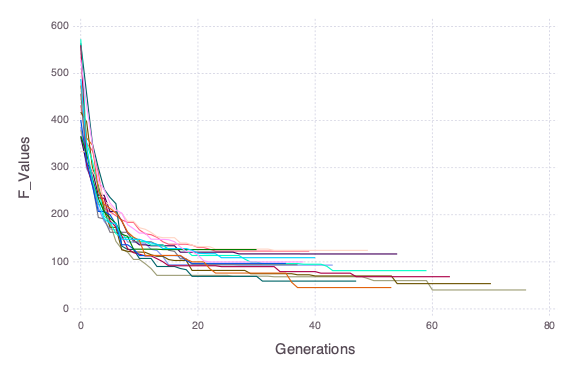
\includegraphics[scale=0.6]{figuras/config_file_5_Rastrigin.png}
	\caption{Primera ejecución}
    \label{fig:primera_ejecucion}
\end{figure}

En la Figura \ref{fig:primera_ejecucion} se ve el resultado de ejecutar el algoritmo 15 veces con la configuración anterior.
Se puede ver como los mejores resultados se obtienen en las primeras generaciones. La mayoría de las ejecuciones muestran como la mejora
del fitness disminuye alrededor de la generación 15-20. Esto puede indicar que cuanto mayor es la generación menor es la diversidad. 
Para apoyar esta idea tenemos las Figuras \ref{fig:best_f_value} y \ref{fig:worst_f_value}. 

La Figura \ref{fig:best_f_value} muestra la diversidad de la ejecución que resulta en un mejor fitness. De la generación 0 a la 30 se produce un decremento de la entropía,
pero se vuelve a recuperar en el resto de generaciones. La entroía empezando y acabando casi con el mismo valor nos dice que el algoritmo mantiene una diversidad similar a 
lo largo de toda la ejecución, lo que puede dar lugar a mejores resultados. En la Figura \ref{fig:worst_f_value}, que muestra la peor ejecución, podemos 
ver un comportamiento similar, el descenso también se produce en las generaciones 0-25. 

\begin{table}[]
    \begin{tabular}{|c|c|c|c|c|c|}
    \hline
                             & \textbf{Evals. de f} & \textbf{Entropía} & \textbf{Distancia de edición} & \textbf{Mejor f} & \textbf{Generaciones} \\ \hline
    \textbf{Mejor ejecución} & 11873                      & 2.69              & 6.20                          & 40.27                     & 77                    \\ \hline
    \textbf{Peor ejecución}  & 4900                       & 2.11              & 5.95                          & 126.14                    & 31                    \\ \hline
    \end{tabular}
    \caption{Comparación de la mejor y la peor ejecución}
    \label{fig:Comparación}
\end{table}

En ambas imágenes la distancia de edición mantiene una correlación estrecha con el valor del fitness, y en ambos casos acaba con unos valores similares. Mirando la tabla \ref{fig:Comparación}, y las figuras
mencionadas no se puede concluir una diferencia clave que marque el por qué una es la mejor ejecución y otra la peor.

\begin{figure}[]
	\centering	
	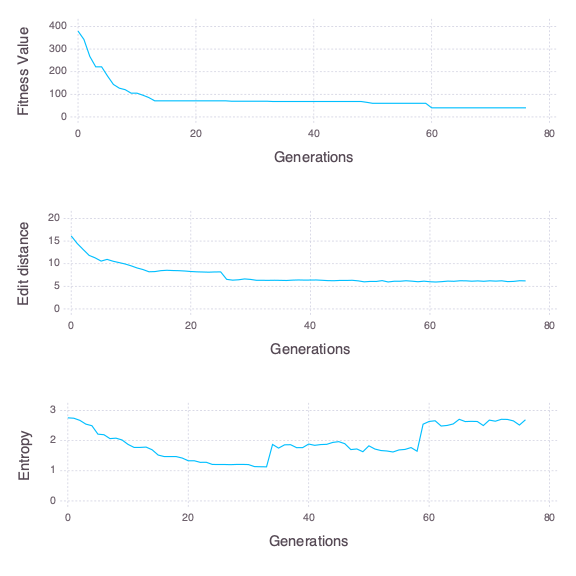
\includegraphics[scale=0.5]{figuras/config_file_5_Rastrigin_best_f_value.png}
	\caption{ Diversidad en la ejecución con mejor resultado de fitness }
    \label{fig:best_f_value}
\end{figure}

\begin{figure}[]
	\centering	
	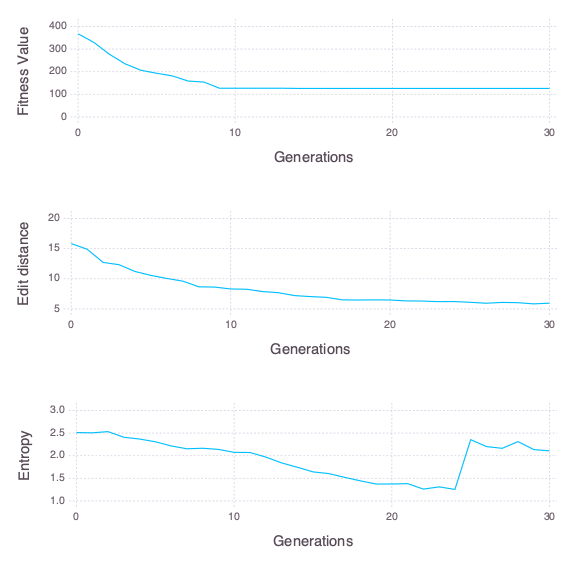
\includegraphics[scale=0.5]{figuras/config_file_5_Rastrigin_worst_f_value.png}
	\caption{ Diversidad en la ejecución con peor resultado de fitness }
    \label{fig:worst_f_value}
\end{figure}

\section{Exploración inicial}

El objetivo de esta exploración es escoger los parámetros: dimensión del cromosoma (\textit{DIM}) y tamaño de población. Primero se varía la dimensión
del cromosoma y la población se mantiene fija a 100. Se ejecutará el algoritmo 15 veces por cada dimensión del cromosoma, y se cogerá el que 
tenga mejor resultado para la comparación. Los resultados de esta primera exploración se encuentran en la Tabla \ref{tab:fitness_variation}. 

\begin{table}[]
    \centering
    \begin{tabular}{||c|c|c|c|c|c||}
        \hline
        \textbf{Fichero Configuración} & \textbf{Generaciones} & \textbf{DIM} & \textbf{Tiempo de ejecución} & \textbf{Mejor fitness} & \textbf{Evals. de f}\\ \hline
        Config File 1   & 16    & 2   & 4.6873  & -76.93    &  2340  \\ \hline
        Config File 2   & 20    & 3   & 7.830   & -74.70    &  2900  \\ \hline
        Config File 3   & 20    & 5   & 4.137   & -67.58    &  2900  \\ \hline
        Config File 4   & 56    & 10  & 5.160   & -45.74    &  8567  \\ \hline
        Config File 5   & 68    & 68  & 4.978   & 49.43     &  10494 \\ \hline
        Config File 6   & 52    & 40  & 4.194   & 422.26    &  8133  \\ \hline
    \end{tabular}
    \caption{Resultados exploración inicial}
    \label{tab:fitness_variation}
\end{table}

Para un tamaño de población 100 aparentemente la mejor dimensión es la 3. Sin embargo, mirando la Figura \ref{fig:box_plots} vemos
que la configuración 2 apenas ha explorado el espacio, ha alcanzado un óptimo local, al igual que la 1 a la 3. Para
futuras explotaciones descartaremos estas configuraciones, ya que no aportan apenas información sobre el comportamiento del algoritmo.
Con la información extraída de estos experimentos no se puede concluir qué valores para tamaño de población ni dimensión del cromosoma 
escoger. En las siguientes secciones se le dará un enfoque diferente. Primero se buscará un valor de
tamaño de población base, que luego variará proporcionalmente con la dimensión.

\begin{figure}[]
	\centering	
	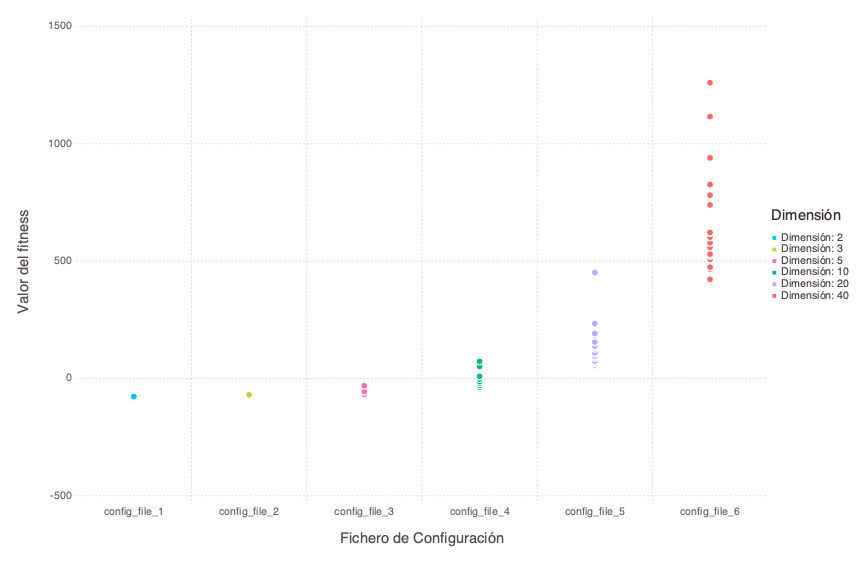
\includegraphics[scale=0.4]{figuras/config_file_1-6_Rastrigin_box_plots.png}
	\caption{ Variación del valor del fitness }
    \label{fig:box_plots}
\end{figure}

\section{Exploración población inicial base}

El objetivo de esta sección es obtener una población inicial base para las próximas exploraciones. Dejaremos fija la dimensión del cromosoma,
será tamaño 2. Se ha escogido esta dimensión porque en la Figura \ref{fig:box_plots} es la que tiene menor mediana.




\begin{table}[]
    \centering
    \begin{tabular}{||c|c|c|c|c||}
        \hline
        \textbf{Fichero Configuración} & \textbf{Generaciones} & \textbf{Tamaño de la población} & \textbf{Mejor fitness} \\ \hline
        Config File 1   & 30    & 5.1160  & 2039.487   \\ \hline
        Config File 7   & 41    & 5.4659  & 1989.754   \\ \hline
        Config File 8   & 32    & 5.1378  & 2068.954   \\ \hline
        Config File 9   & 42    & 4.9277  & 1971.862   \\ \hline
        Config File 10   & 46    & 4.7593  & 2059.756   \\ \hline
    \end{tabular}
    \caption{Resultados exploración inicial}
    \label{tab:base_population}
\end{table}



\section{Análisis de las soluciones}

- en que casos da mejor resultado y por qué, comparar con hipótesis inicial
- Por qué da mejores resultados con una función o con otra o con respecto al algoritmo genético

\subsection{Con Búsqueda Local}

% TODO: hacer la misma tabla para diferentes tamaños de población
\begin{tabular}{||c|c|c|c|c||}
    \hline
    \textbf{Fichero Configuración} & \textbf{Función} & \textbf{DIM} & \textbf{Tiempo de ejecución} & \textbf{Mejor elemento} \\ \hline
    example                                     & example          & 2      & example                      & example                 \\ \hline
                                                &                  & 3             &                              &                         \\ \hline
                                                &                  & 5             &                              &                         \\ \hline
                                                &                  & 10             &                              &                         \\ \hline
                                                &                  & 20             &                              &                         \\ \hline
                                                &                  & 40             &                              &                         \\ \hline

\end{tabular}

